\documentclass[12pt,spanish]{article}
\usepackage[spanish]{babel}
\usepackage{graphicx}
\usepackage{color}
\usepackage{xcolor}
\usepackage{colortbl}
\usepackage{amsthm,thmtools}
\usepackage{dirtytalk}
\usepackage{multirow}
\usepackage{amsmath}
\usepackage{subcaption}
\usepackage{adjustbox}
\usepackage{amsmath}
\usepackage{centernot}
\usepackage{mathtools}
\usepackage{multirow}
\usepackage[hidelinks]{hyperref}
\usepackage{caption}
\usepackage{eurosym} % para el euro
\usepackage{amsthm}
\usepackage{multicol}
\usepackage{float}
\usepackage{amsfonts}
\usepackage{apacite}

\usepackage{titling}
\usepackage{soul}
\usepackage{listings}
\usepackage{array}
\usepackage{tikz}
\usetikzlibrary{shapes.geometric, arrows, chains, calc,positioning,fit,decorations.pathreplacing}
\usepackage[framemethod=tikz]{mdframed}

\graphicspath{ {../img/}}
\selectlanguage{spanish}
\usepackage[utf8]{inputenc}
\usepackage{graphicx}
\usepackage[a4paper,left=3cm,right=2cm,top=2.5cm,bottom=2.5cm]{geometry}

\newenvironment{solution}{
	\par
	\textbf{Solución}
	\par
	\begin{center}
}
{
	\end{center}
}

\lstset{
  breaklines=true,
  postbreak=\mbox{\textcolor{red}{$\hookrightarrow$}\space},
}


\title{Servidores Web de Altas Prestaciones}
\setlength{\droptitle}{10em}
\author{Carlos Sánchez Páez}

\makeindex
\begin{document}
\definecolor{light-gray}{gray}{0.95}
\lstset{columns=fullflexible,basicstyle=\ttfamily}
\surroundwithmdframed[
  hidealllines=true,
  backgroundcolor=light-gray,
  innerleftmargin=0pt,
  innertopmargin=0pt,
  innerbottommargin=0pt]{lstlisting}


\begin{titlepage}

 \newlength{\centeroffset}
 \setlength{\centeroffset}{-0.5\oddsidemargin}
 \addtolength{\centeroffset}{0.5\evensidemargin}
 \thispagestyle{empty}

 \noindent\hspace*{\centeroffset}
 \begin{minipage}{\textwidth}

  \centering
  
\includegraphics[width=0.9\textwidth]{logo_ugr.jpg}\\[1.4cm]

  \textsc{ \Large Servidores Web de Altas Prestaciones\\[0.2cm]}
  \textsc{GRADO EN INGENIERÍA INFORMÁTICA}\\[1cm]

  {\Huge\bfseries T5: Desplegando una granja web en Google Cloud Platform \\}
	{\Large Horas dedicadas: 6 \\}

 \end{minipage}

 \vspace{1.5cm}
 \noindent\hspace*{\centeroffset}
 \begin{minipage}{\textwidth}
  \centering

  \textbf{Autor}\\ {Carlos Sánchez Páez}\\[2.5ex]
  
\includegraphics[width=0.4\textwidth]{etsiit_logo.png}\\[0.1cm]
  \vspace{1.5cm}
  
\includegraphics[width=0.15\textwidth]{atc.jpg}\\[0.1cm]
  \vspace{1cm}
  \textsc{Escuela Técnica Superior de Ingenierías Informática y de Telecomunicación}\\
  \vspace{1cm}
  \textsc{Curso 2019-2020}
 \end{minipage}
\end{titlepage}
\thispagestyle{empty}
\newpage
\tableofcontents{}
\newpage


\section{Introducción}

En este proyecto desplegaremos la siguiente arquitectura en \cite{GCP}.

\begin{figure}[H]
	\centering
	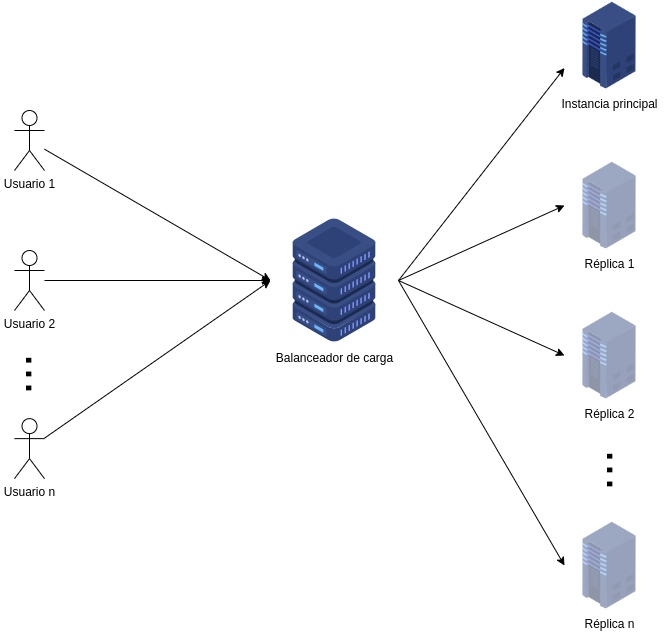
\includegraphics[width=0.5\textwidth]{project/architecture.png}
	\caption{Esquema de la granja web a desplegar}
\end{figure}

Nuestra granja contará con una instancia principal (servidor web) que se servirá a partir del balanceador de carga. Cuando ésta incremente, se crearán nuevas instancias y la carga se distribuirá entre ellas. El objetivo principal es que los usuarios sólo conozcan la dirección del balanceador de carga, no las de los servidores finales.
\newpage
\section{¿Qué es Google Cloud Platform?}

\emph{Google Cloud Platform (GCP)} es un conjunto de recursos de computación que el propio \emph{Google} utiliza para ofrecer sus productos (\emph{Youtube}, \emph{Translate}, \emph{Search}, etc.). Es la tercera empresa mundial en el mercado de servidores en la nube o \emph{Cloud Computing} (tras \emph{Amazon Web Services} y \emph{Microsoft Azure}). Ofrece Infraestructura como Servicio (\emph{IaaS}), Software como Servicio\emph{SaaS} y Plataforma como Servicio \emph{SaaS} mediante sus más de 50 productos.

\subsection{Ventajas de Google Cloud Platfom}

Los principales puntos fuertes de este servicio son los siguientes:
\begin{itemize}
	\item Proporciona tutoriales interactivos (mediante \href{https://www.qwiklabs.com/}{https://www.qwiklabs.com/}) para iniciarse en el uso de la plataforma de manera sencilla.
	\item Incluye un panel de control con gran cantidad de estadísticas y métricas sobre nuestro proyecto, instancia, red, etc. para facilitar la monitorización.
	\item Existen aplicaciones de GCP para Android e iOS, por lo que se puede acceder al panel de control desde cualquier lugar.
	\item Ofrece una prueba gratuita por un valor de 300\$.
	\item Cuenta con una terminal web y una herramienta CLI (\emph{gcloud}) para manejar la plataforma (crear instancias, redes, etc.).
\end{itemize}

\begin{figure}[H]
  \begin{subfigure}[t]{0.5\textwidth}
    \centering
		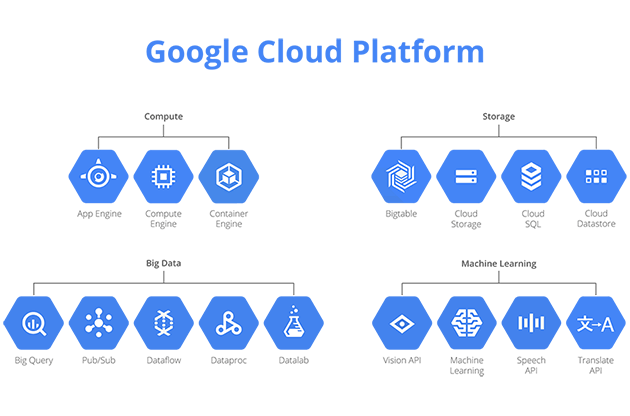
\includegraphics[width=\textwidth]{project/gcp_products.png}
  \end{subfigure}
  \hspace{0.5cm}
  \begin{subfigure}[t]{0.5\textwidth}
    \centering
		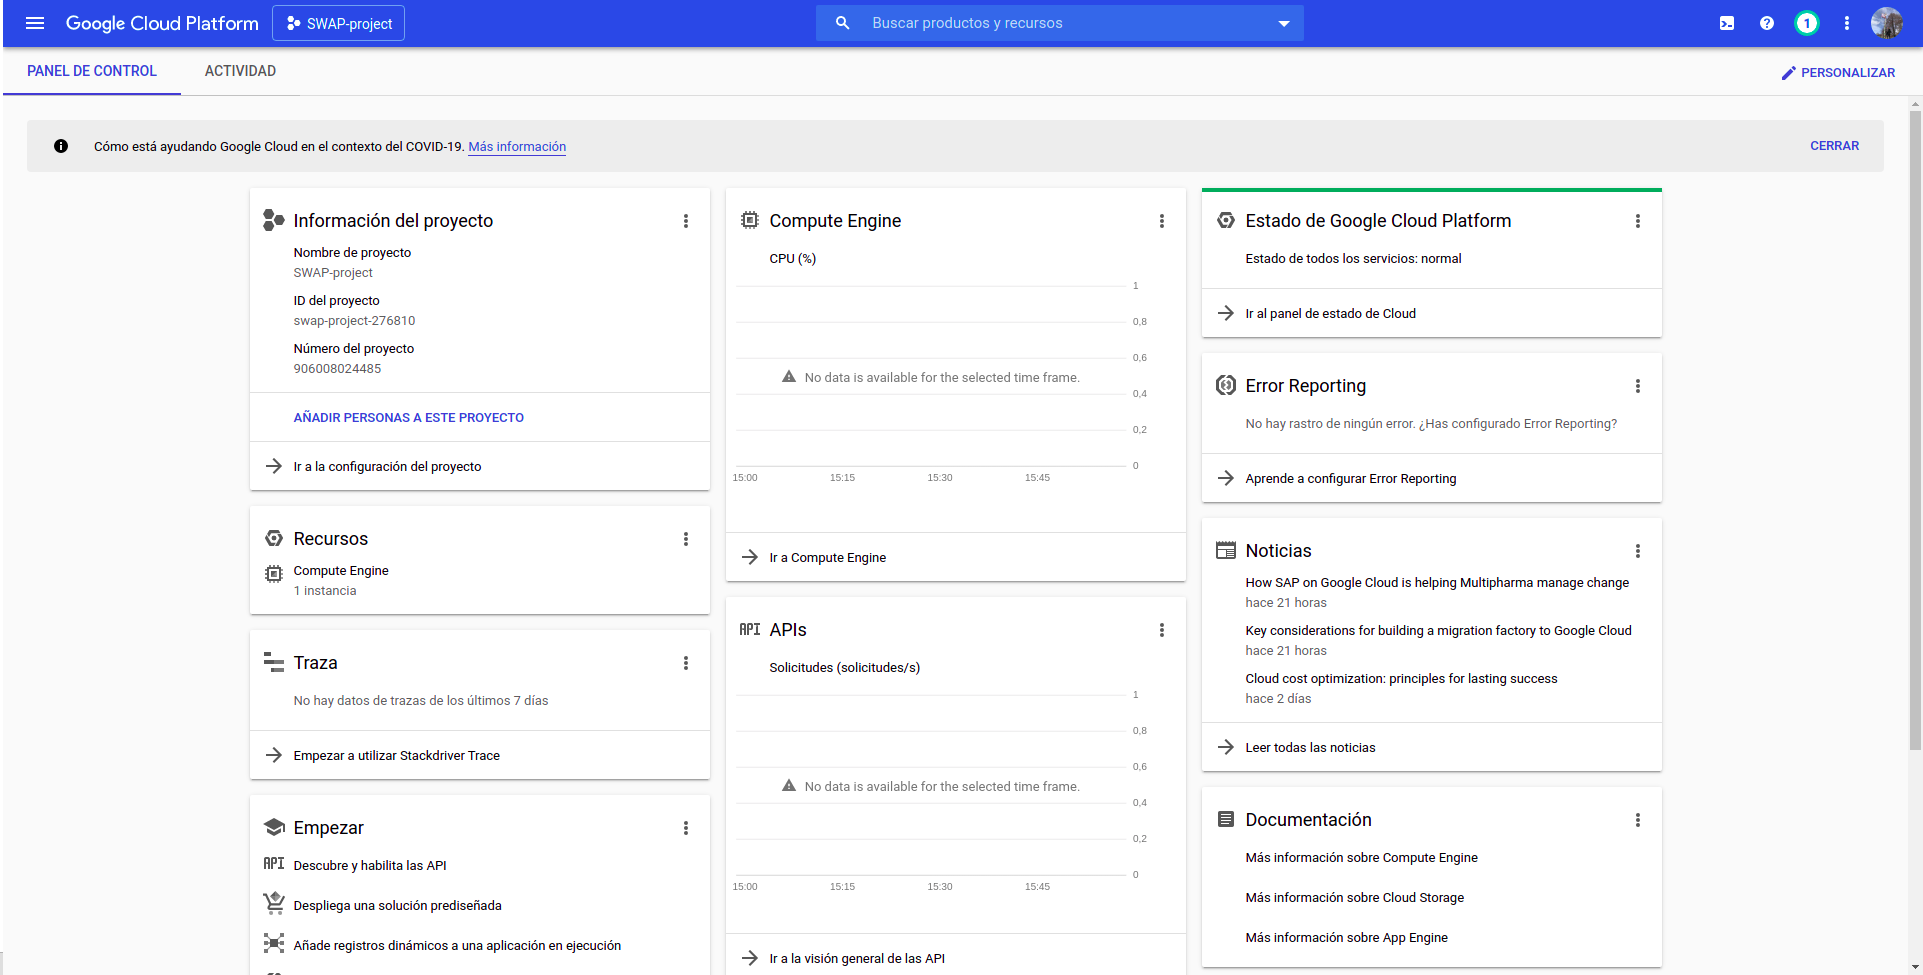
\includegraphics[width=\textwidth]{project/controlpanel.png}
  \end{subfigure}
	\caption{Productos y Panel de Control de GCP}
\end{figure}
\newpage
\subsection{Empresas que utilizan Google Cloud Platform}

Algunas de las entidades más famosas que utilizan este servicio son:
\begin{itemize}
 \item New York Times.
 \item Twitter.
 \item Ebay.
 \item Telenor.
 \item Paypal.
\end{itemize}

\begin{figure}[H]
	\centering
	
\includegraphics[width=0.5\textwidth]{project/logos.png}
	\caption{Empresas que usan GCP}
\end{figure}

En este proyecto nos centraremos en la herramienta \emph{Compute Engine} (\emph{IaaS}) para desplegar una granja web de servidores HTTP. Esta granja contará con \emph{autoescalado}. Es decir, cuando se someta a una carga alta, se crearán nuevas instancias y el balanceador de carga distribuirá el trabajo entre ellas. Cuando se llegue a un período de relajación, las nuevas instancias que se crearon se eliminarán para ahorrar costes.

\newpage
\section{Despliegue de la granja web}

\begin{enumerate}
	\item Comenzamos conectándonos a la plataforma con nuestra cuenta de Google mediante el siguiente enlace: (\href{https://console.cloud.google.com/}{https://console.cloud.google.com/})
	\item Creamos un proyecto y le damos un nombre:
	\begin{figure}[H]
		\centering
		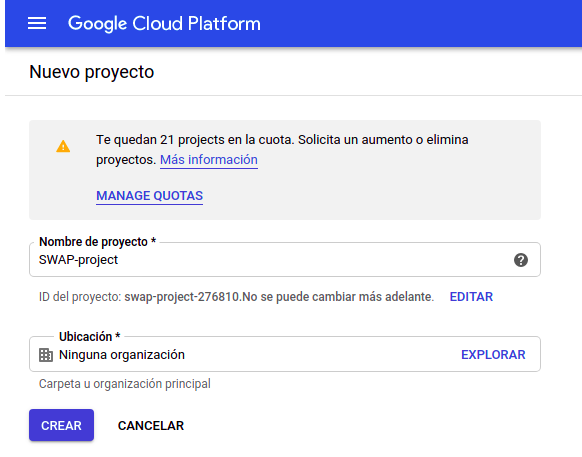
\includegraphics[width=0.6\textwidth]{project/create_project.png}
		\caption{Creación del proyecto}
	\end{figure}
	\item Creamos una red para los servidores web (Redes $\implies$ Redes VPC):
	\begin{figure}[H]
		\centering
		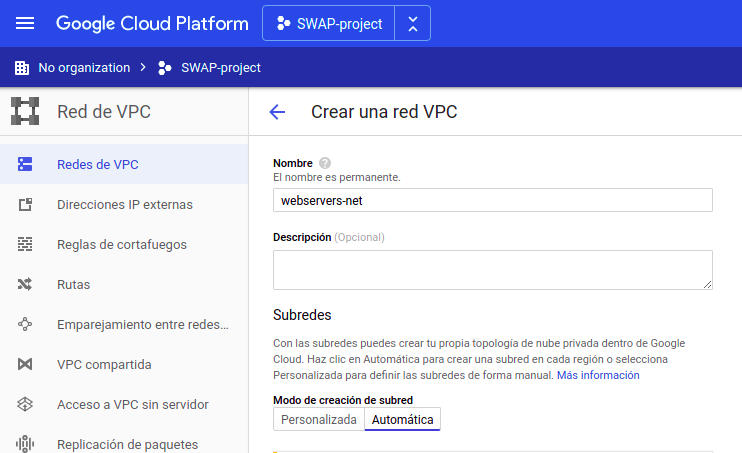
\includegraphics[width=0.6\textwidth]{project/vpc_creation.png}
		\caption{Creación de la VPC para los servidores finales}
	\end{figure}
	\newpage
	\item Añadimos una regla de firewall (Redes $\implies$ Reglas de Firewall) a nuestra red y permitimos las conexiones desde cualquier lugar (0.0.0.0/0) al puerto 80 (HTTP):
		\begin{figure}[H]
			\centering
			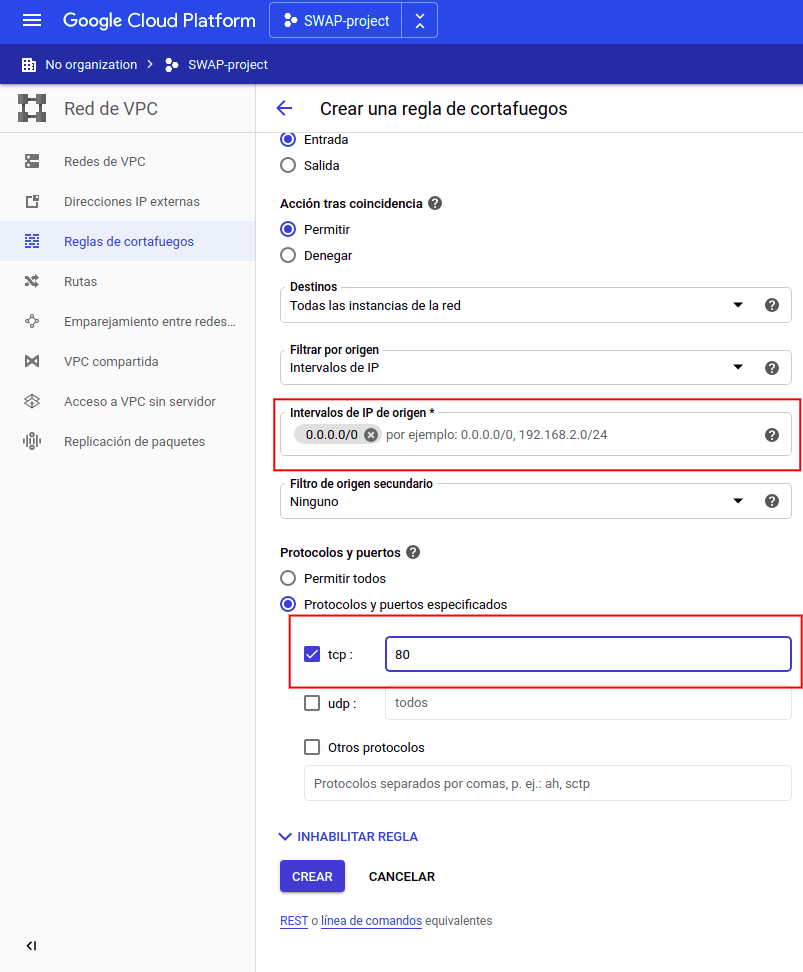
\includegraphics[width=0.5\textwidth]{project/firewall_creation.png}
			\caption{Creación de una regla de firewall que permita todas las conexiones HTTP}
		\end{figure}
	\item Accedemos a la gestión de grupos de instancias (Compute Engine $\implies$ Grupos de instancias) y creamos un grupo gestionado:
	\begin{figure}[H]
		\centering
		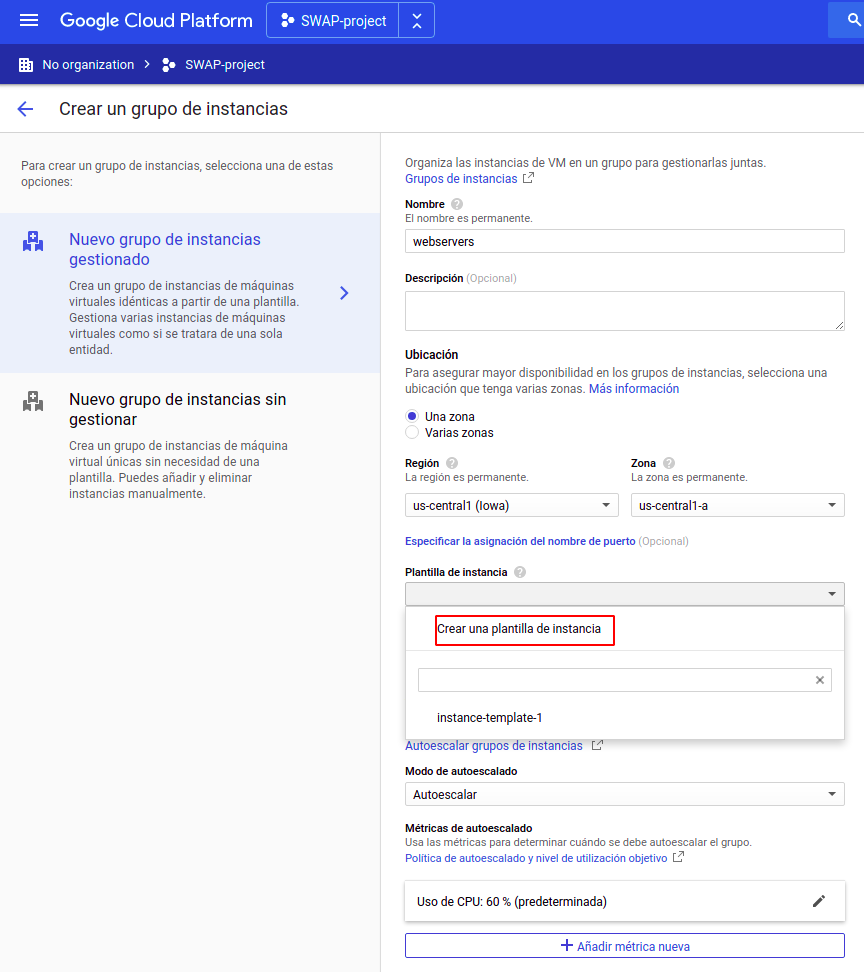
\includegraphics[width=0.5\textwidth]{project/createig.png}
		\caption{Creación del grupo de instancias}
	\end{figure}
	\item Hacemos clic en crear plantilla y elegimos la imagen de Ubuntu 18.04:
	\begin{figure}[H]
		\centering
		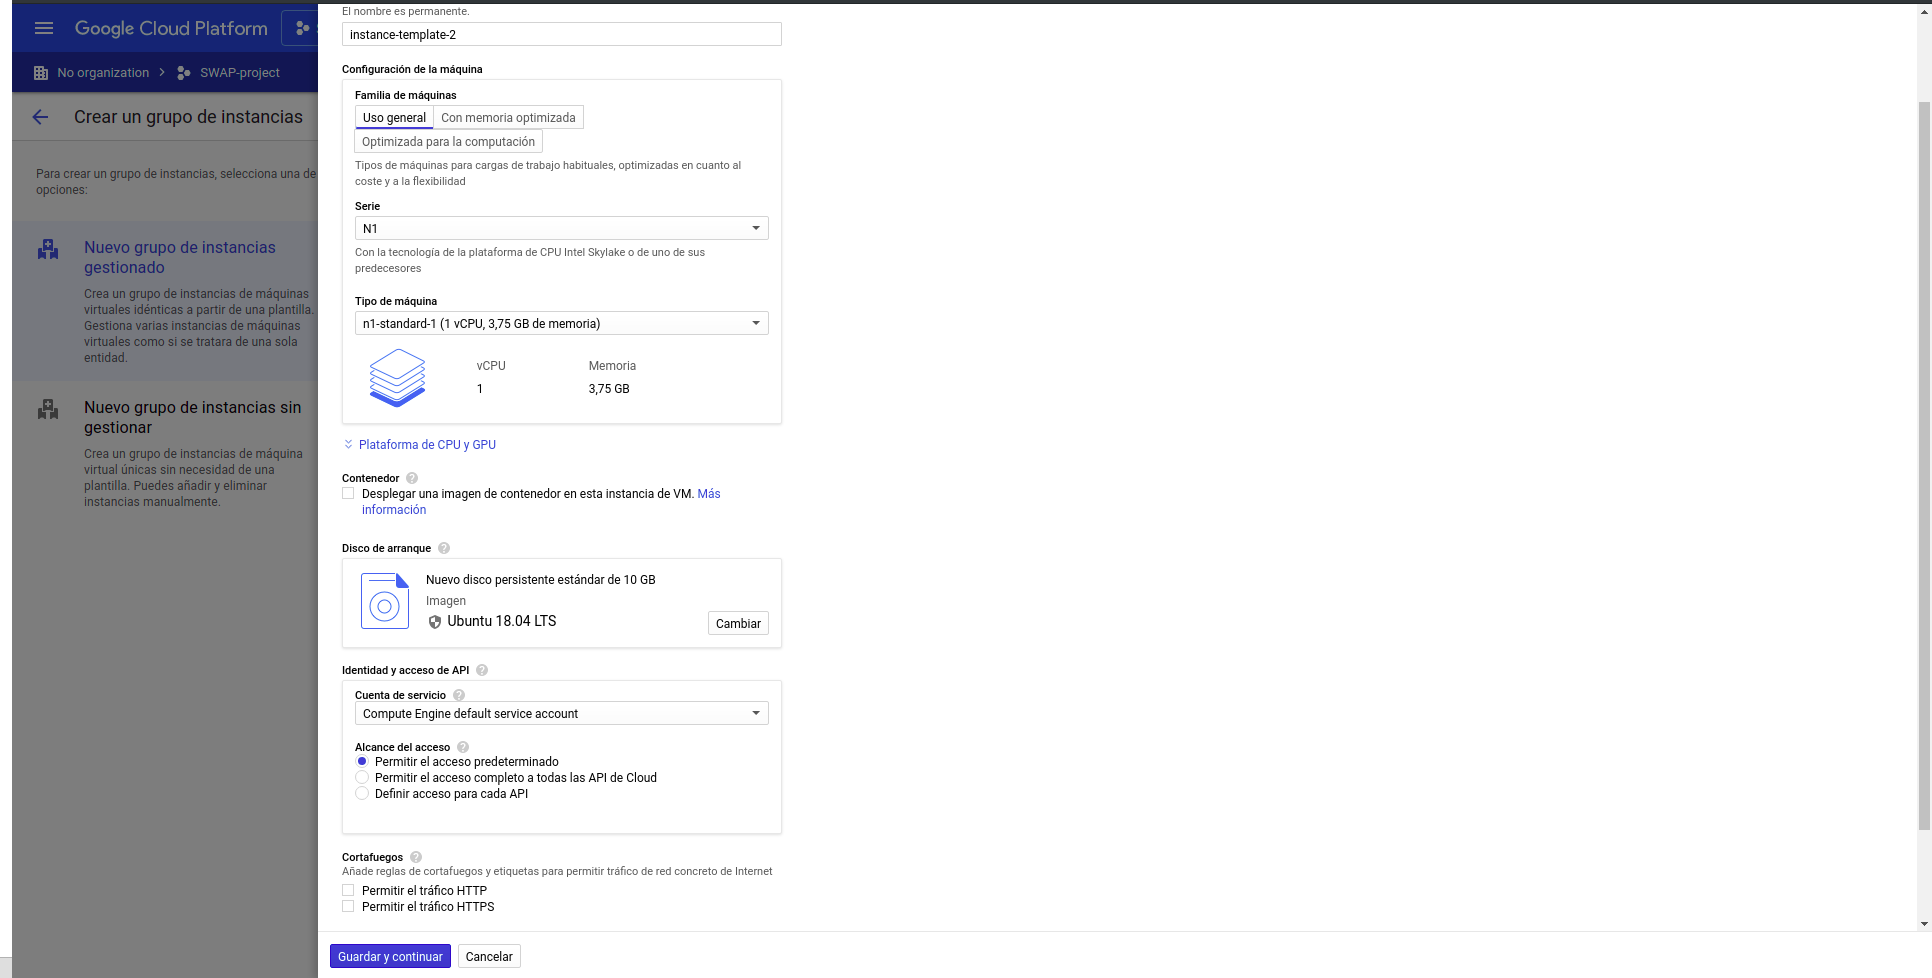
\includegraphics[width=0.5\textwidth]{project/createtemplate.png}
		\caption{Creación de la plantilla con la que se lanzarán las instancias}
	\end{figure}
	\item Hacemos que se instale el servidor web \emph{apache} al inicio de cada instancia:
	\begin{figure}[H]
		\centering
		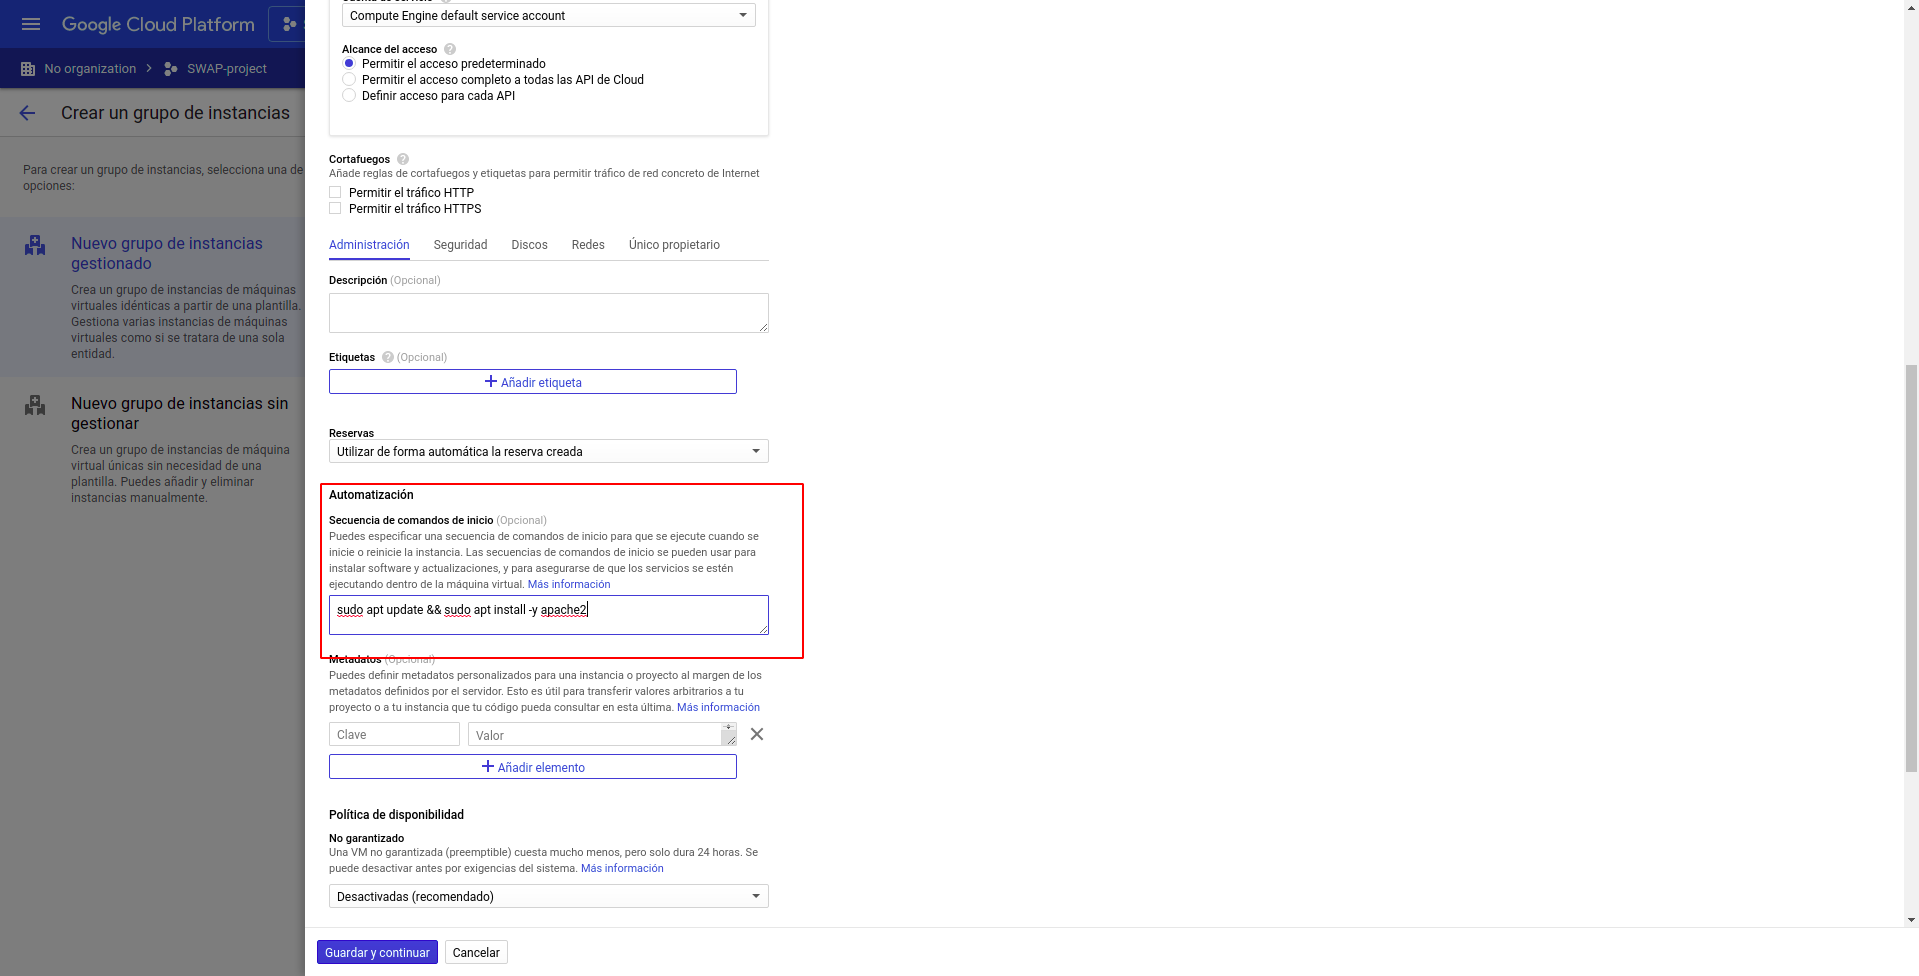
\includegraphics[width=0.5\textwidth]{project/automation.png}
		\caption{Instalación del servidor web al inicio de cada instancia}
	\end{figure}
	\newpage
	\item Asignamos la red que creamos anteriormente a la plantilla:
	\begin{figure}[H]
		\centering
		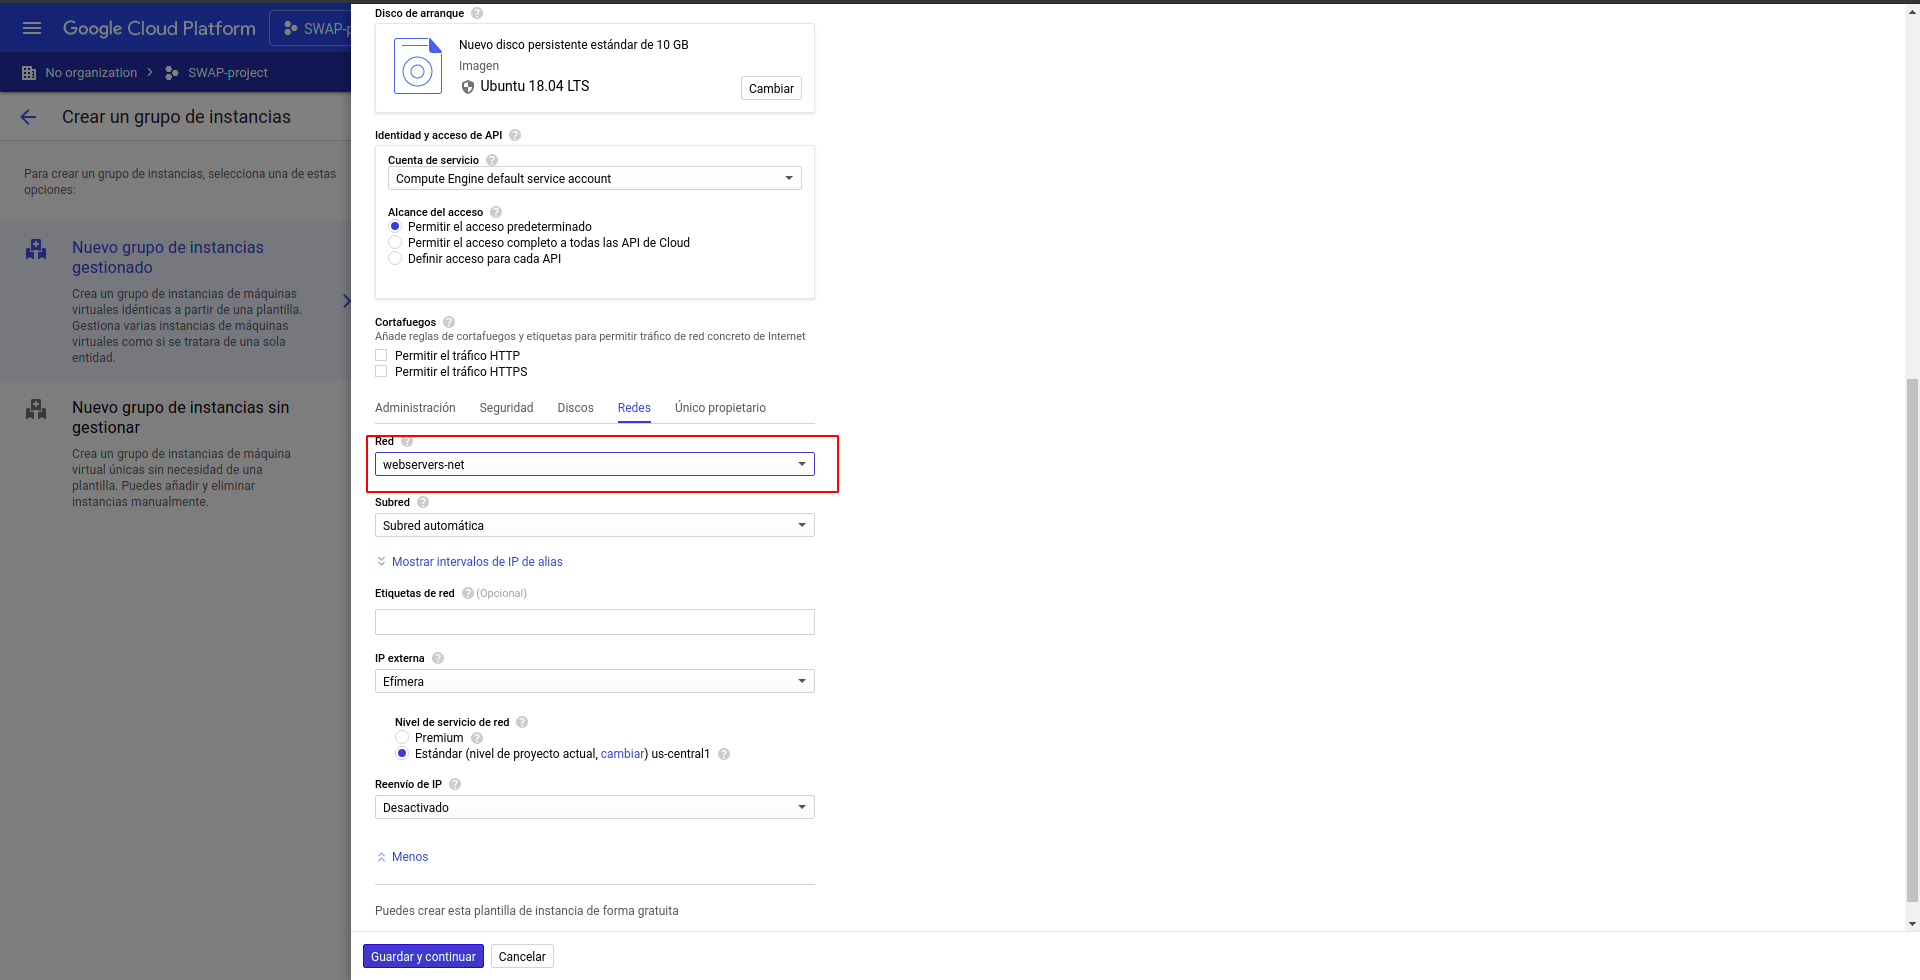
\includegraphics[width=0.5\textwidth]{project/network.png}
		\caption{Asignación de red a las instancias}
	\end{figure}
	\newpage
	\item Pasamos a la creación del balanceador de carga (Servicios de red $\implies$ Balanceo de carga)
	\begin{figure}[H]
		\centering
		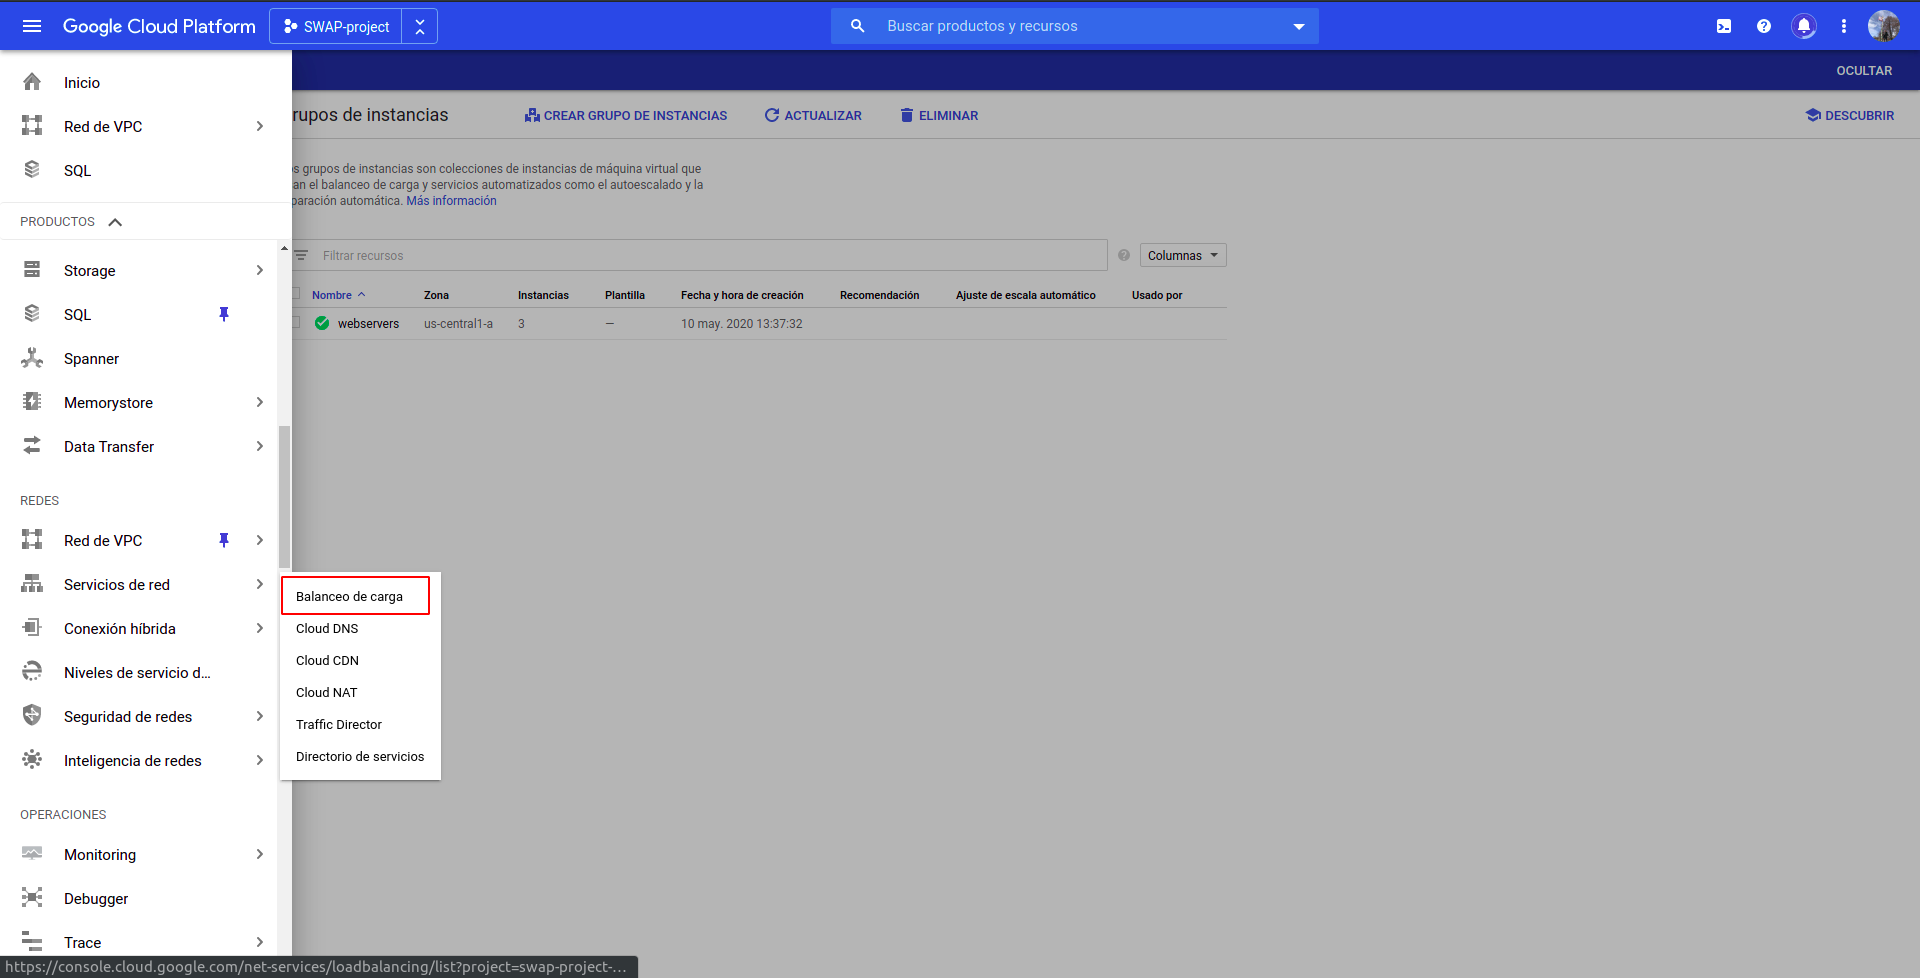
\includegraphics[width=\textwidth]{project/loadbalancer.png}
		\caption{Creación del balanceador de carga}
	\end{figure}
	\item Seleccionamos \emph{Balanceo de carga de HTTP(s)}
	\begin{figure}[H]
		\centering
		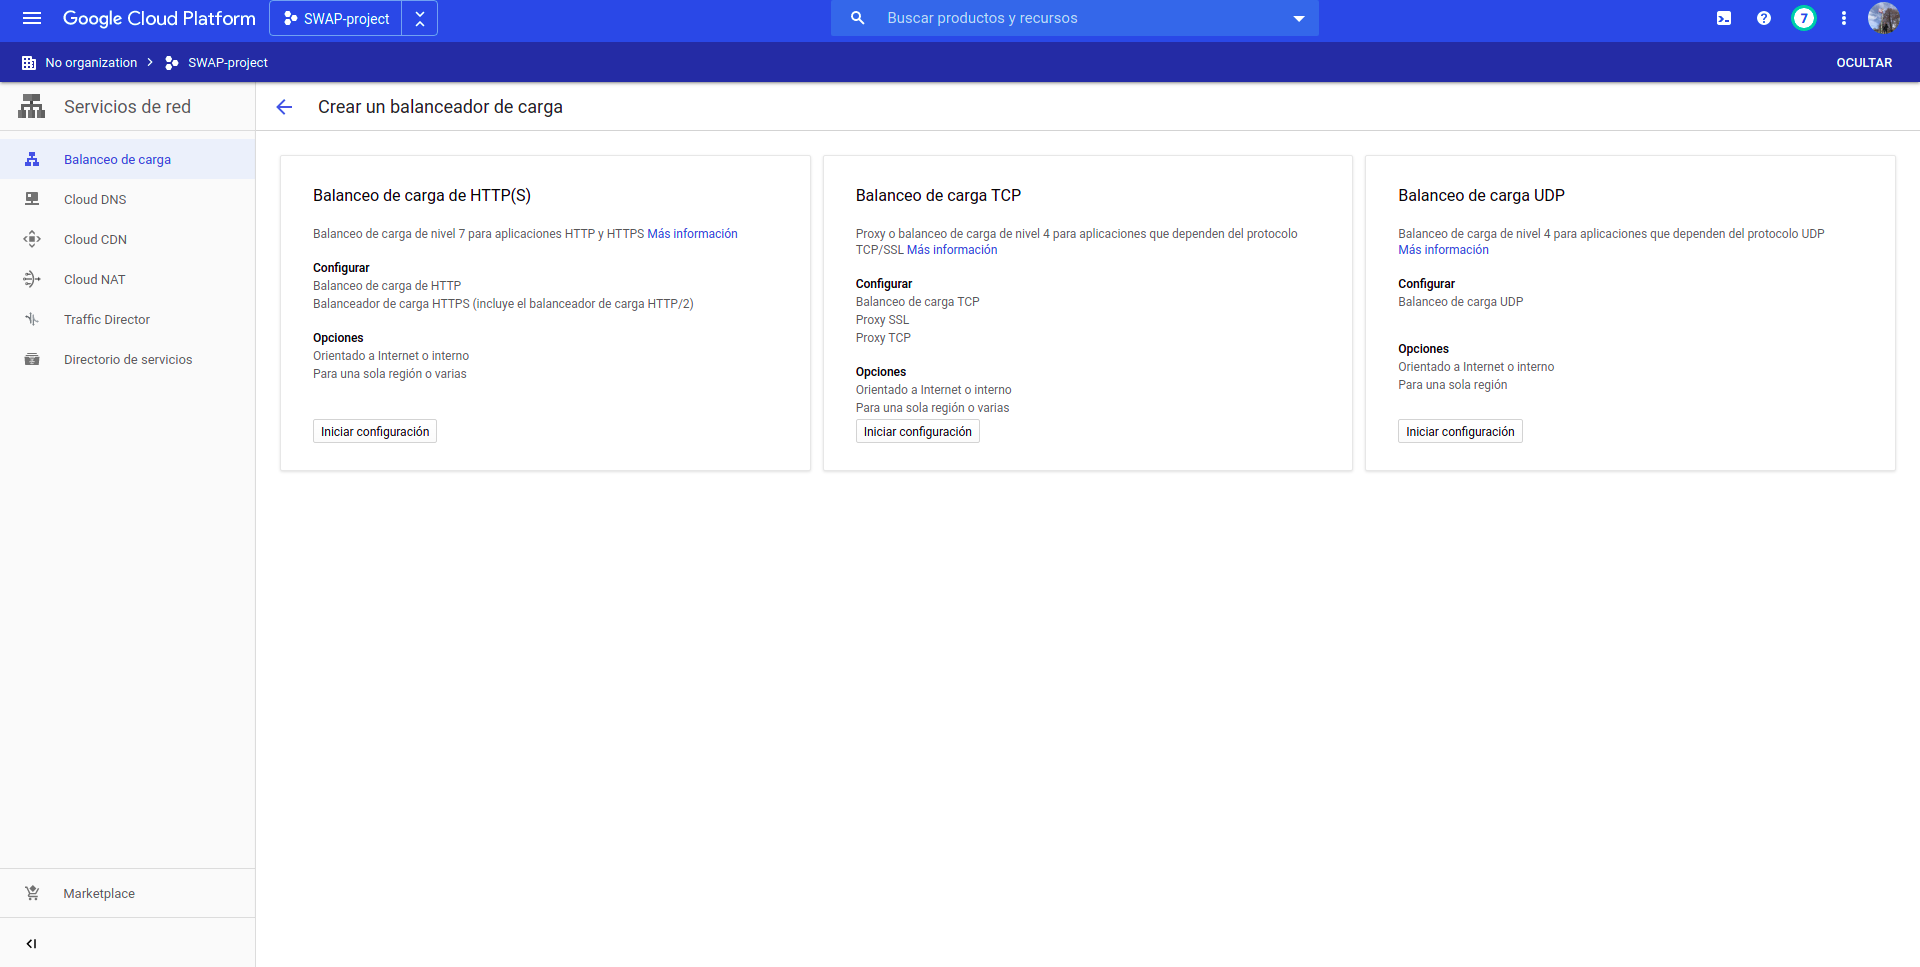
\includegraphics[width=\textwidth]{project/loadbalancerhttps.png}
		\caption{Selección de balanceador de carga HTTP(s)}
	\end{figure}
	\newpage
	\item Elegimos el balanceo desde Internet a las VMs
	\begin{figure}[H]
		\centering
		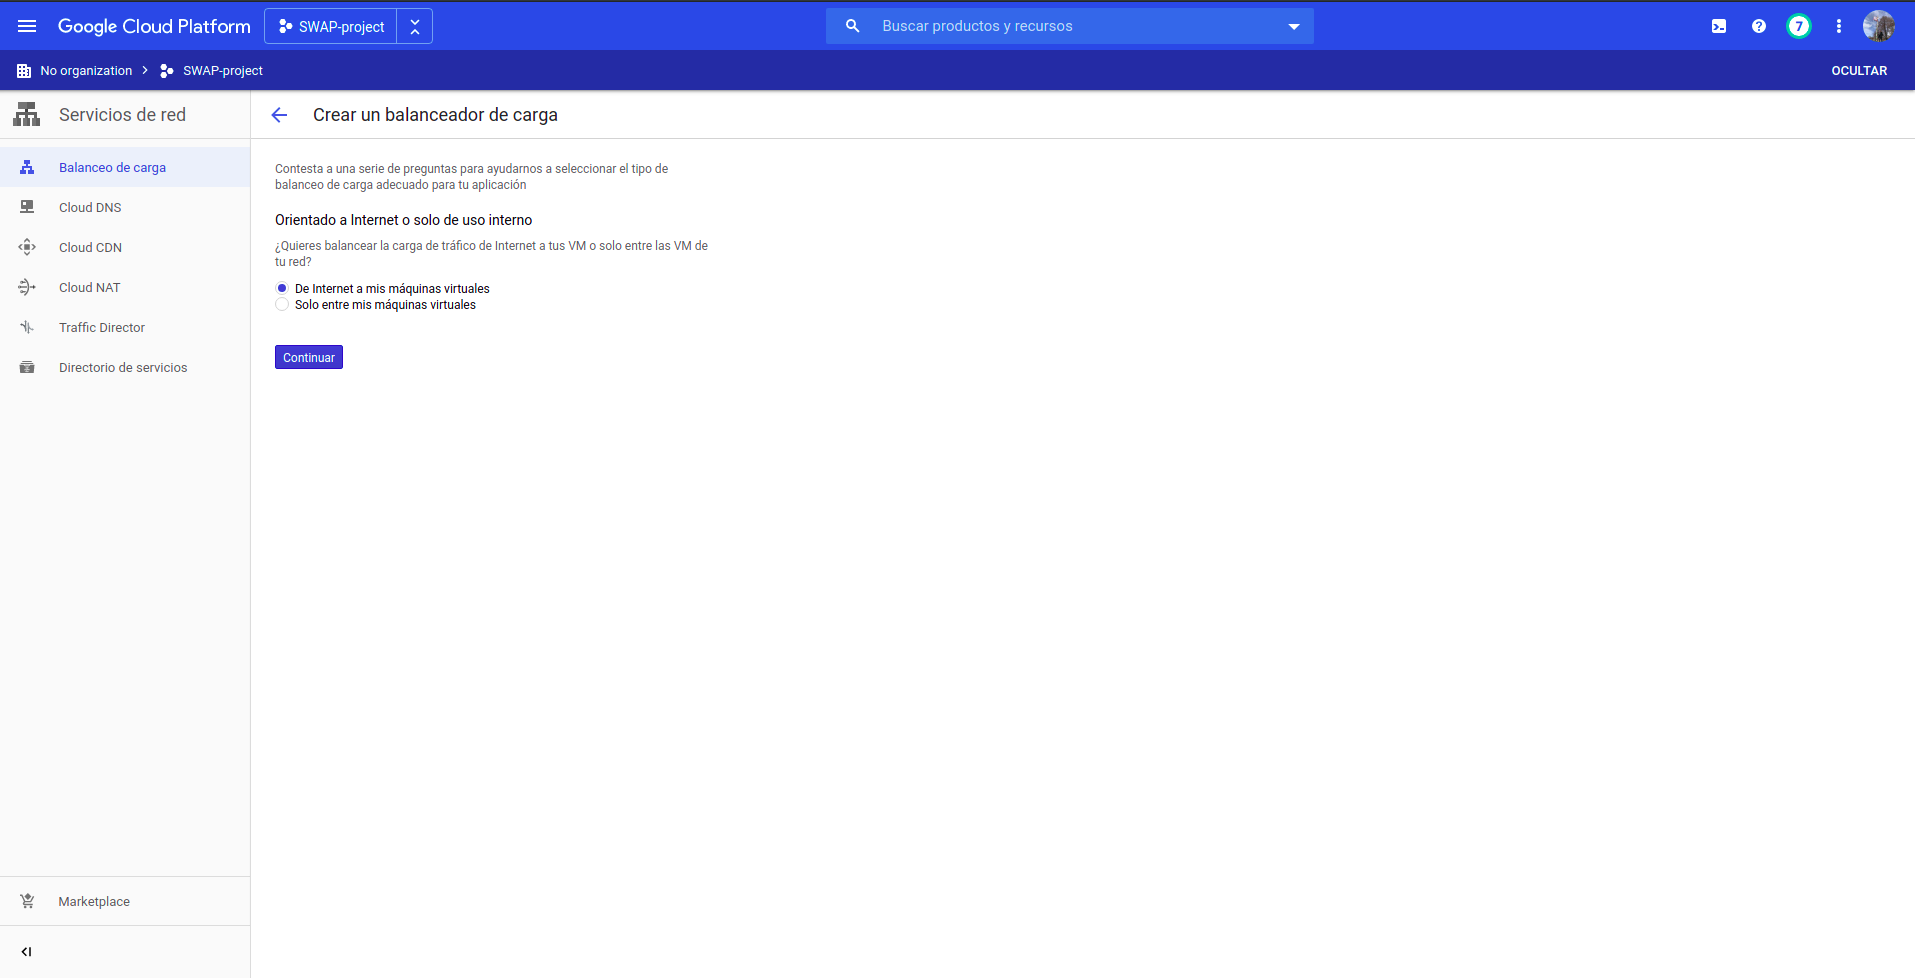
\includegraphics[width=0.8\textwidth]{project/frominternet.png}
		\caption{Elección del tipo de balanceo}
	\end{figure}
	\item Configuramos el backend eligiendo nuestro grupo de instancias:
	\begin{figure}[H]
		\centering
		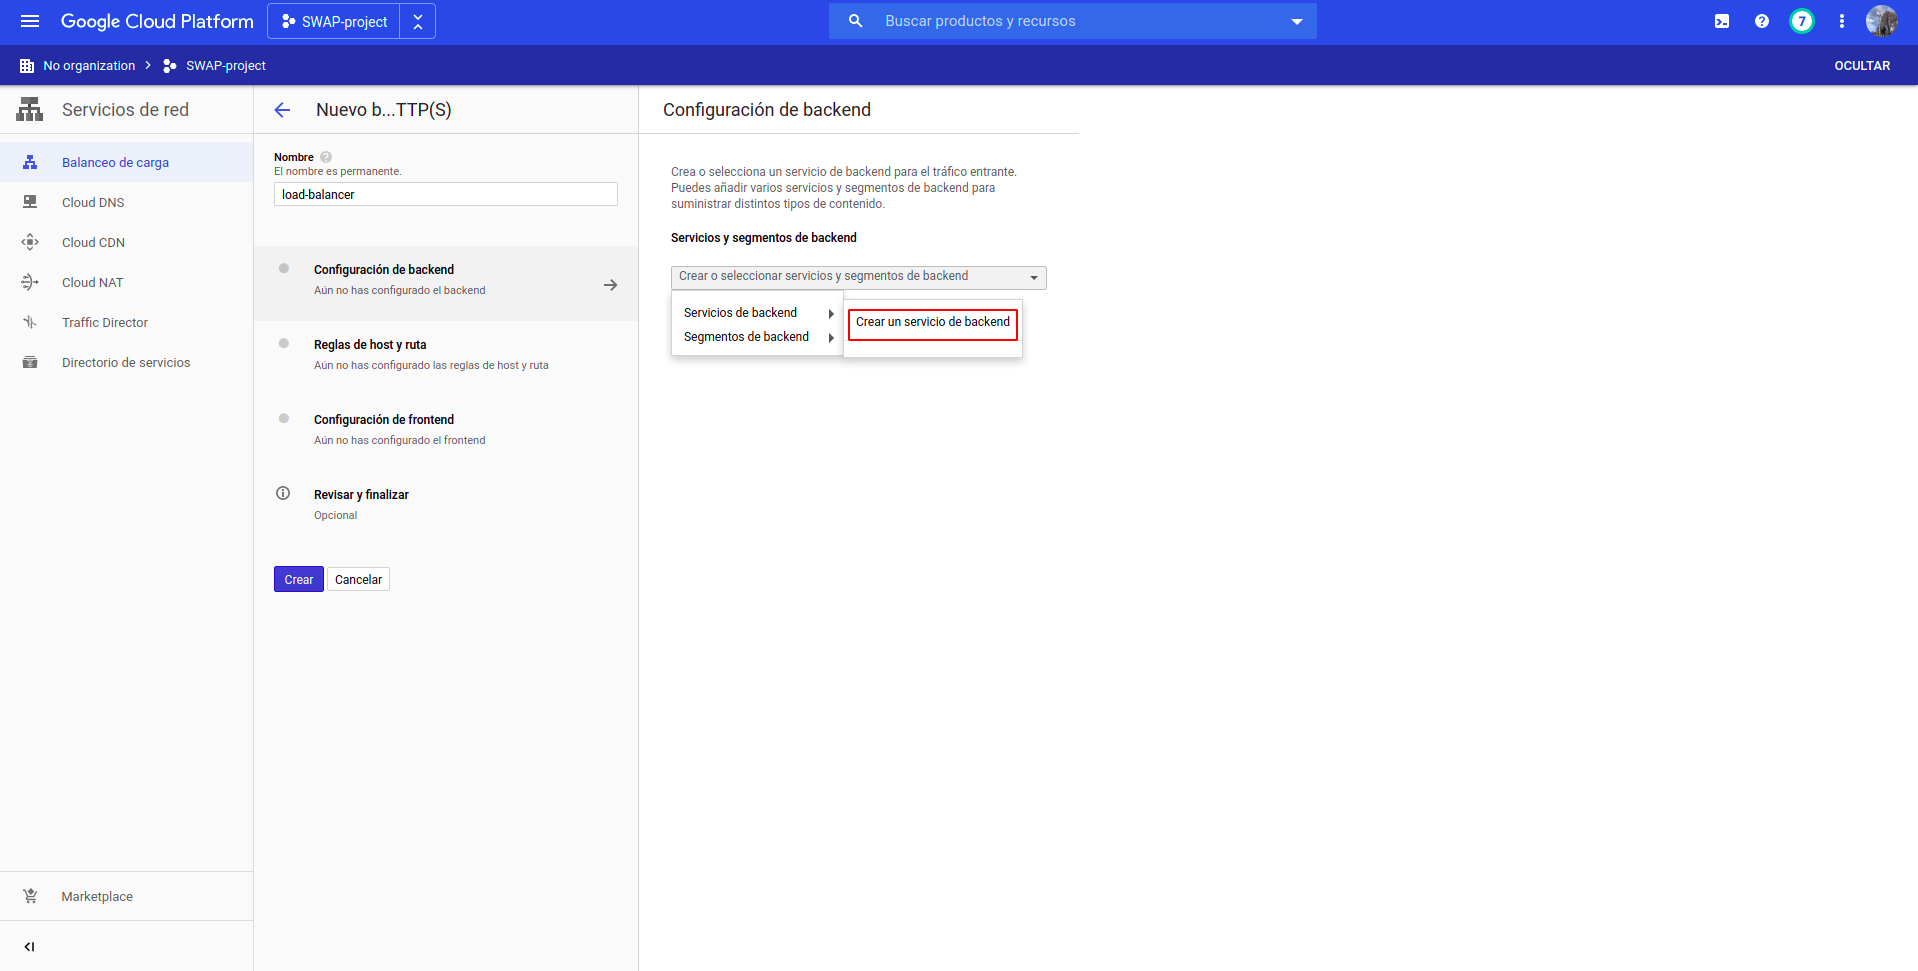
\includegraphics[width=0.8\textwidth]{project/backend.png}
		\caption{Configuración del backend}
	\end{figure}
	\begin{figure}[H]
		\centering
		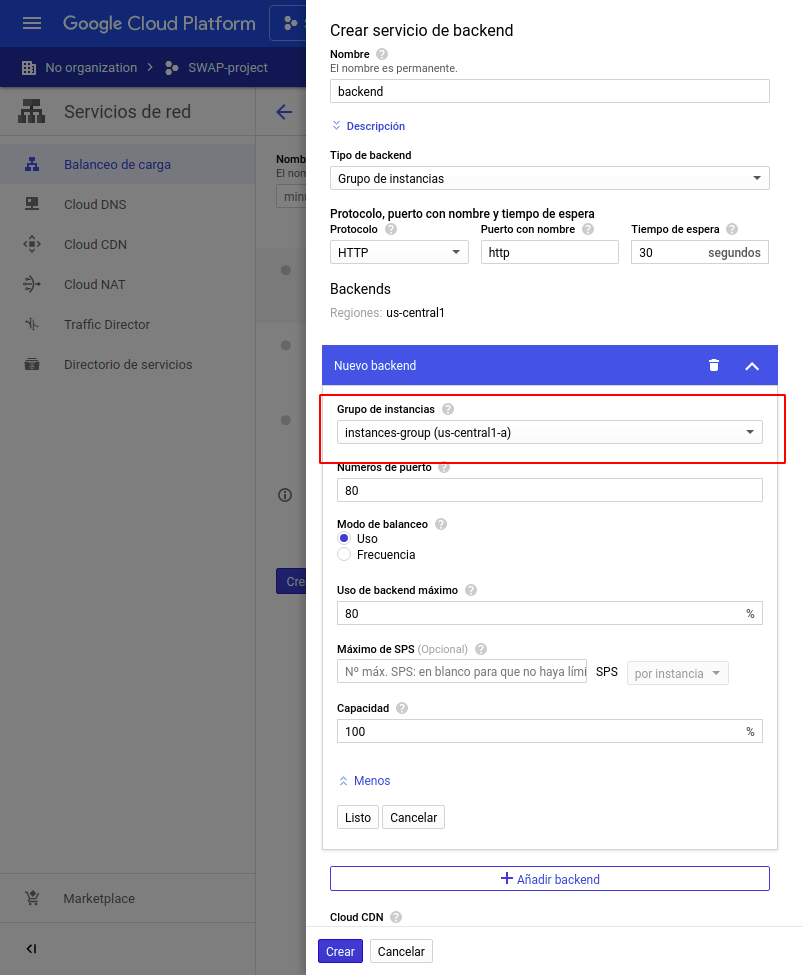
\includegraphics[width=0.8\textwidth]{project/backend_selection.png}
		\caption{Enlace entre backend y grupo de instancias}
	\end{figure}
	\newpage
	\item Creamos una comprobación de estado (determinará si la instancia está disponible y creará una nueva en caso contrario):
	\begin{figure}[H]
		\centering
		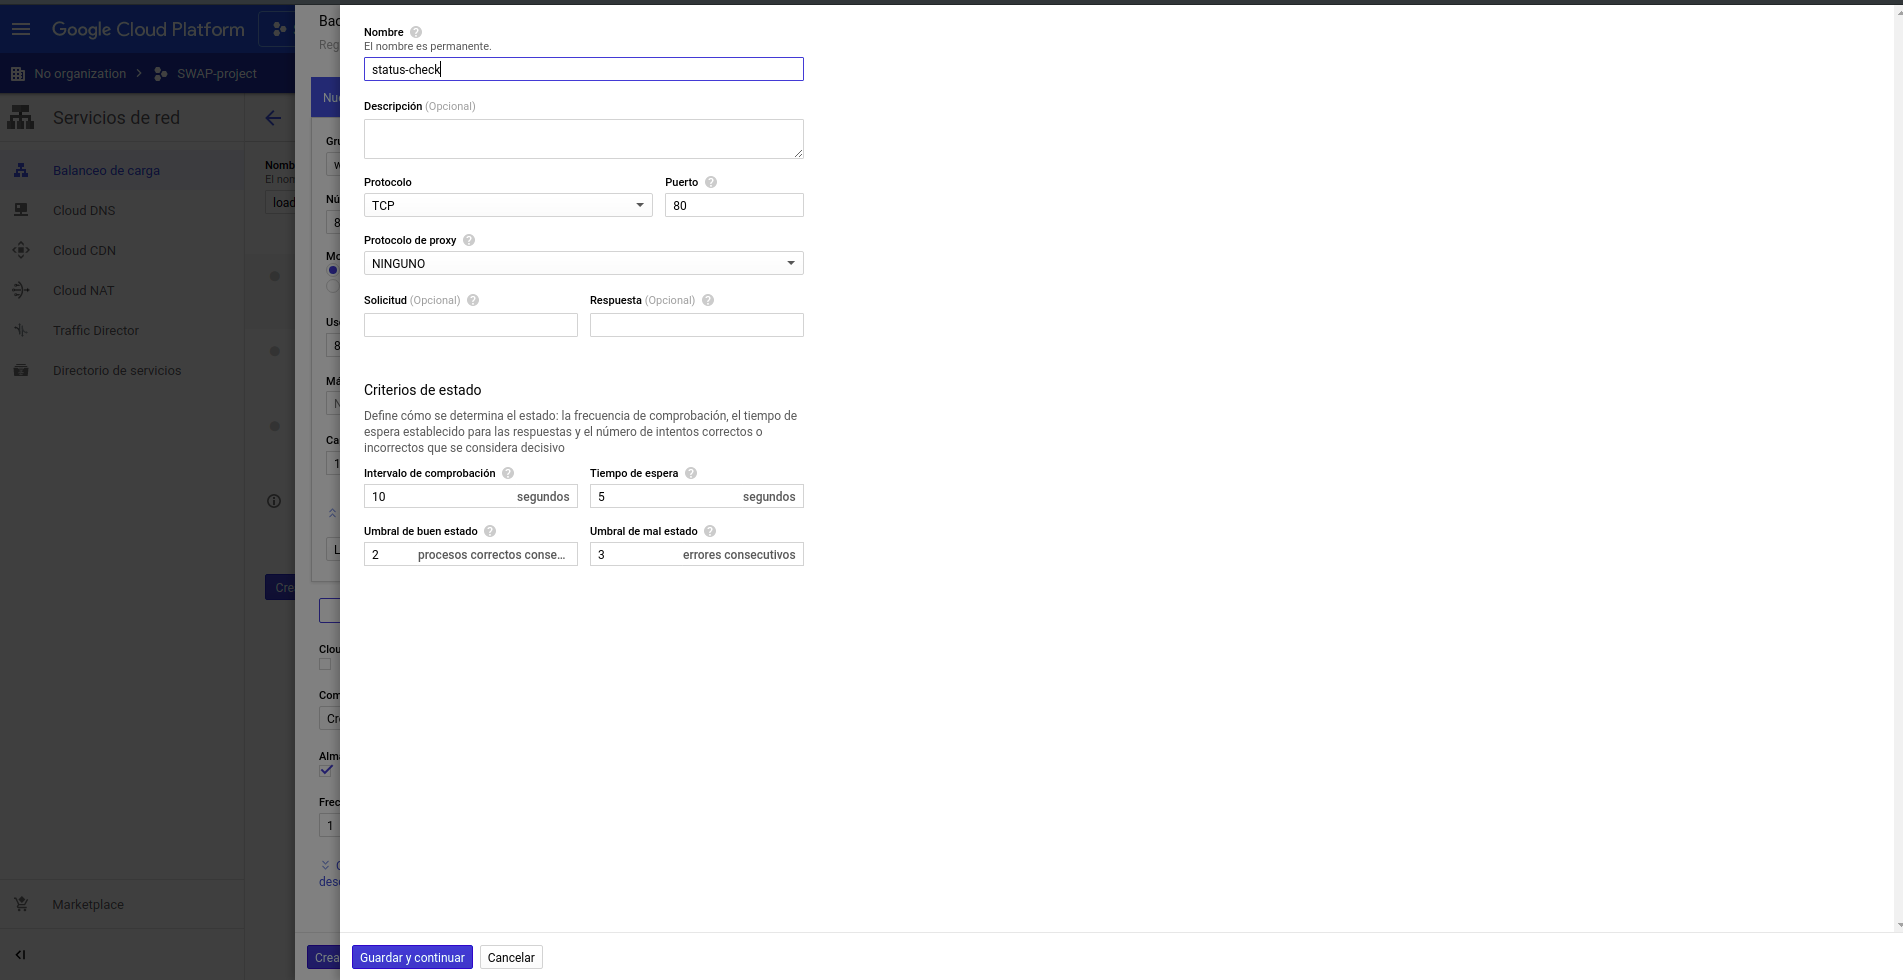
\includegraphics[width=0.5\textwidth]{project/status_check.png}
		\caption{Creación de la comprobación de estado}
	\end{figure}
	\newpage
	\item Pasamos a la configuración del frontend. Le damos nombre y creamos una IP estática:
	\begin{figure}[H]
		\centering
		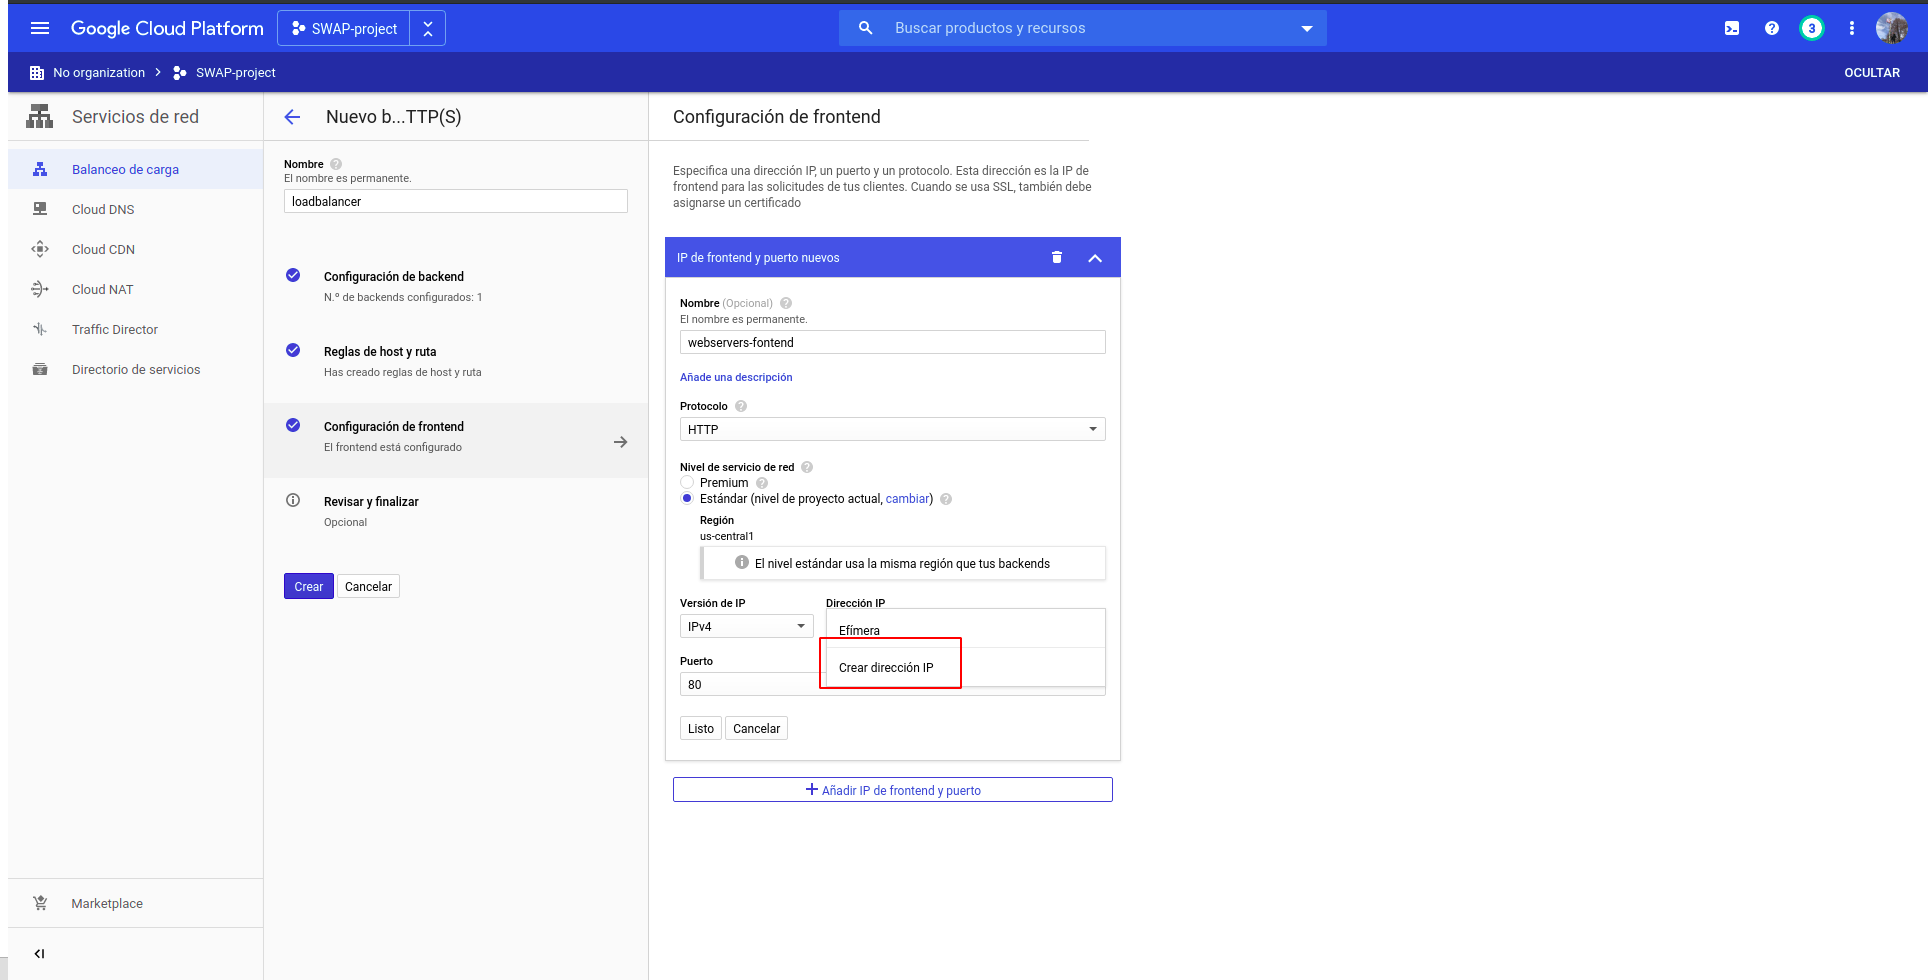
\includegraphics[width=0.8\textwidth]{project/frontend.png}
		\caption{Configuración del frontend}
	\end{figure}
	\item Esperamos a que se cree el balanceador y accedemos a su IP externa para comprobar que funciona:
	\begin{figure}[H]
		\centering
		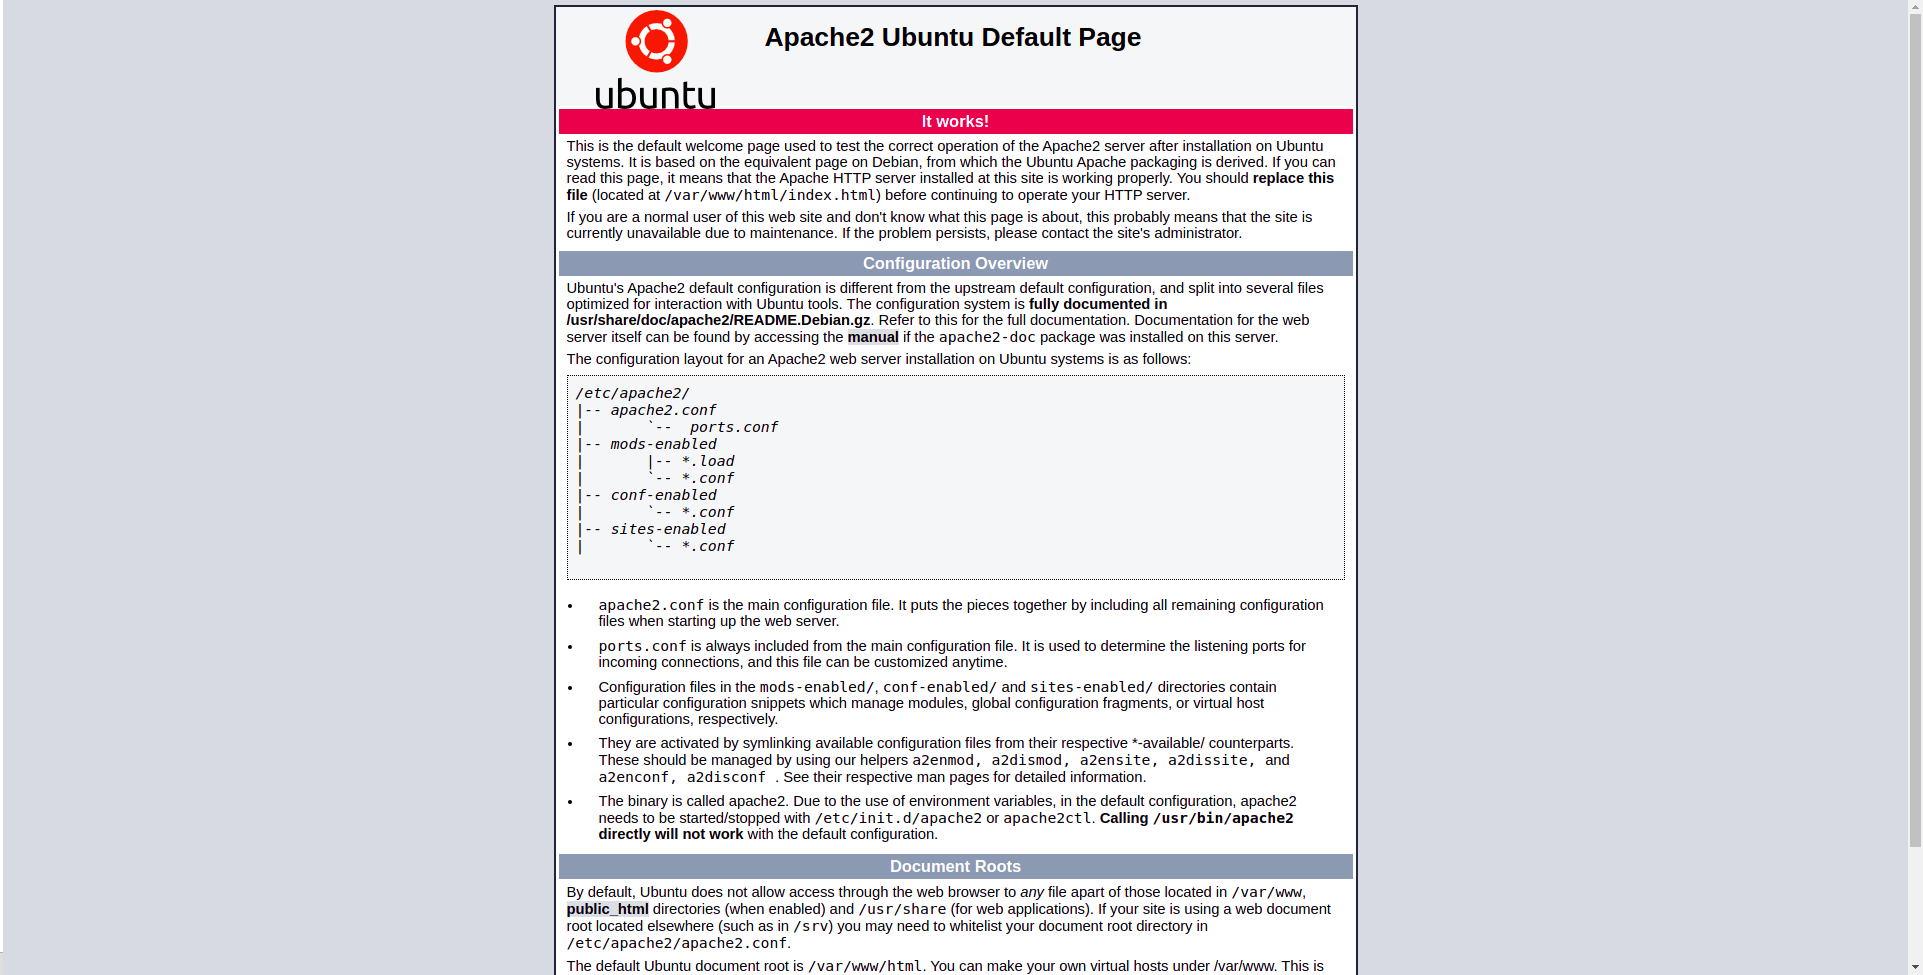
\includegraphics[width=0.8\textwidth]{project/load_balancer_ok.png}
		\caption{Acceso a la dirección del balanceador}
	\end{figure}
	\newpage
	\item Ahora someteremos el balancerador a mucha carga para comprobar que se cean máquinas nuevas. Utilizaremos \emph{Apache Benchmark (ab)} para ello (desde nuestra máquina):
	\begin{figure}[H]
		\centering
		\begin{lstlisting}
		host > ab -n 100000 -c 300 http://35.208.234.230/
		\end{lstlisting}
	\caption{Comando para ejecutar la prueba de estrés}
\end{figure}
	Esto lanzará 100000 peticiones desde 300 usuarios concurrentes contra nuestro balanceador. Lo ejecutamos dos veces y comprobamos la gráfica generada en monitorización:
	\begin{figure}[H]
		\centering
	  \begin{subfigure}[t]{0.8\textwidth}
			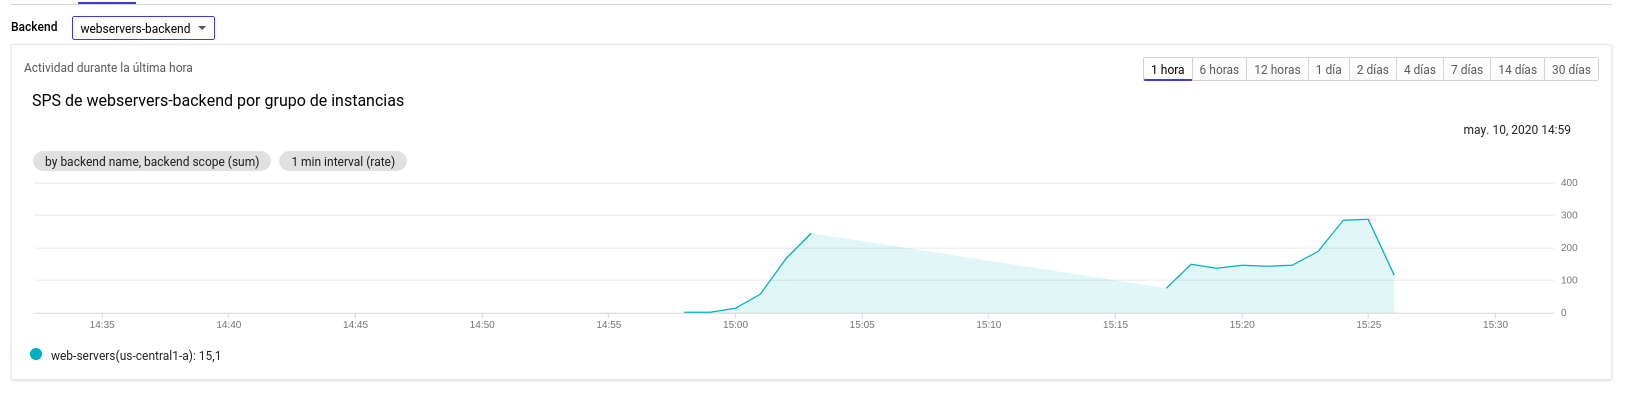
\includegraphics[width=\textwidth]{project/monitoring.png}
			\caption{Monitorización del balanceador de carga}
	  \end{subfigure}
	  \begin{subfigure}[t]{0.8\textwidth}
			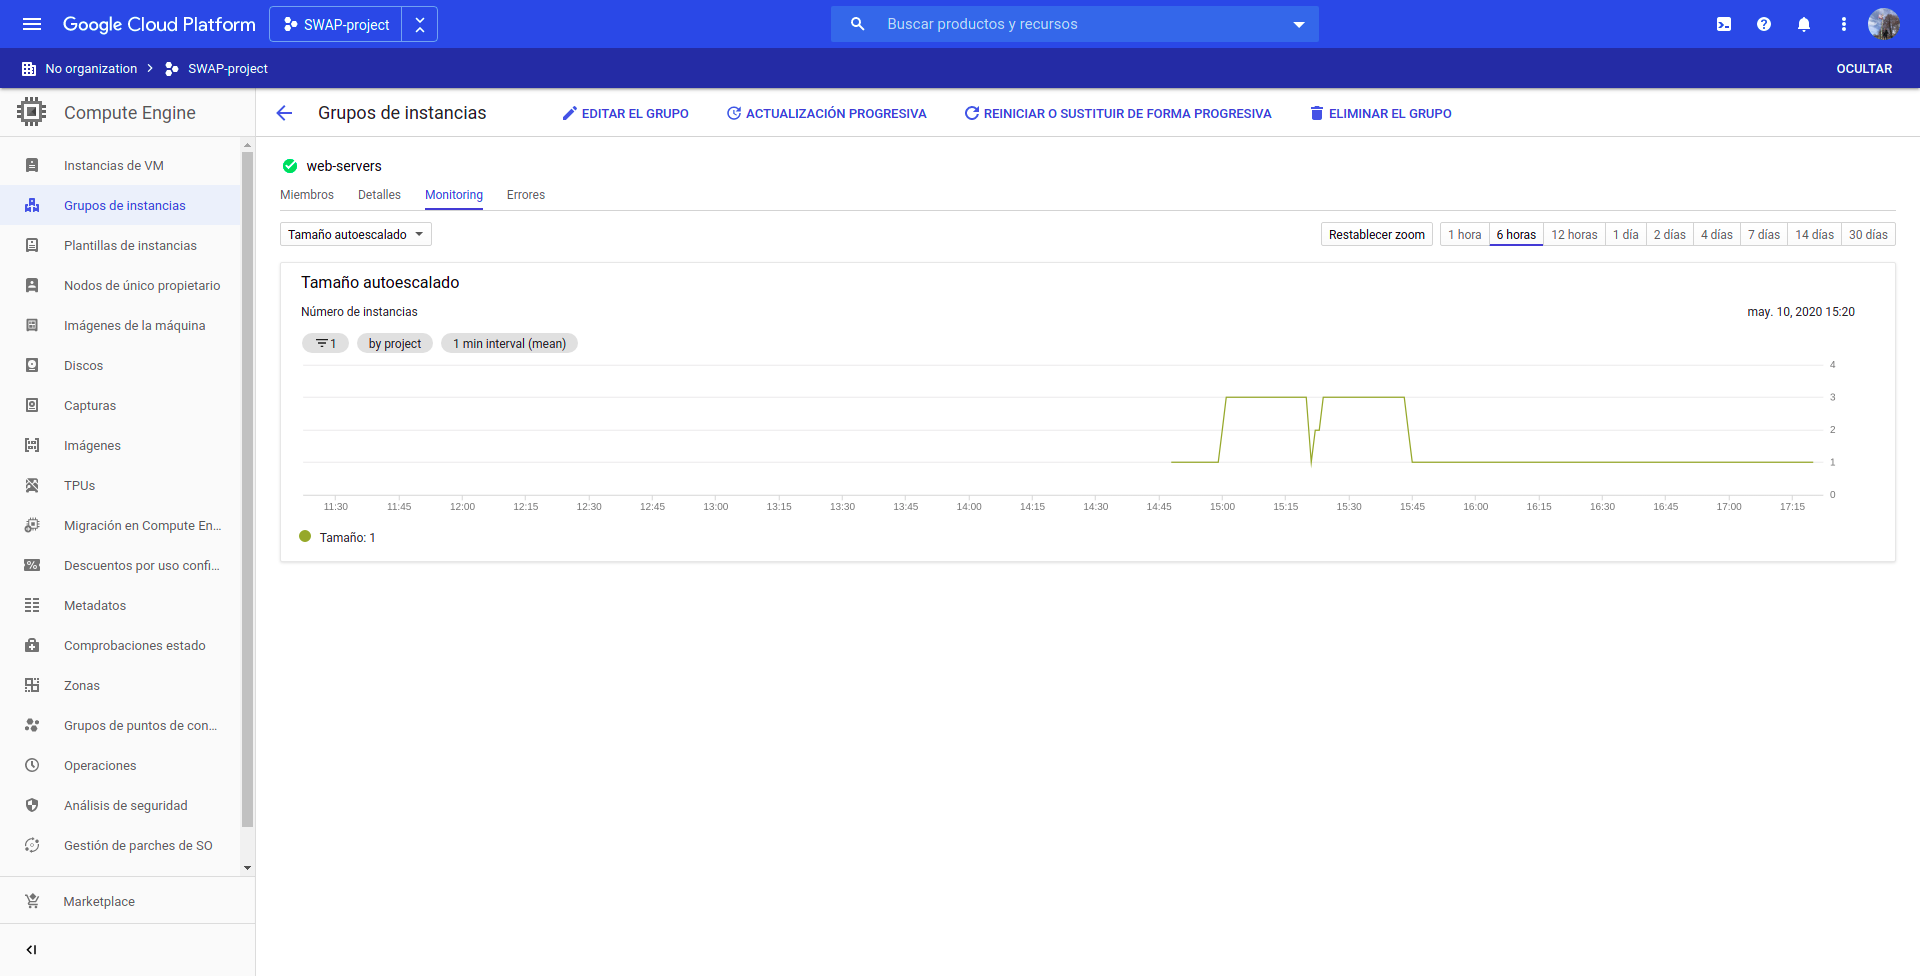
\includegraphics[width=\textwidth]{project/monitoring_groups.png}
			\caption{Monitorización del grupo de instancias}
	  \end{subfigure}
		\caption{Monitorización del sistema tras las pruebas de estrés}
	\end{figure}
	Podemos observar como, al recibir mucha carga, se ha, creado dos instancias más. Cuando hubo un período de relajación (tiempo entre el final del primer test y el comienzo del segundo), se eliminaron esas dos nuevas instancias y se volvieron a crear al inicio de la segunda prueba de estrés.

\end{enumerate}
\newpage
\subsection{Asegurar la granja web}
En el apartado anterior configuramos el firewall para que se pudiera acceder desde cualquier lugar al puerto 80 desde cualquier máquina. En esta sección haremos que sólo podamos conectarnos al balanceador y que las instancias sólo acepten conexiones de éste.
\begin{enumerate}
	\item Vamos a Firewall (Redes $\implies$ Reglas de Firewall) y creamos una regla nueva. Debemos seleccionar nuestra red y todas las instancias que estén en ella. En los rangos IP admitidos añadiremos los del balanceador de carga y los del health-check (https://cloud.google.com/load-balancing/docs/https\#firewall\_rules) en el puerto TCP:80.
	\begin{figure}[H]
		\centering
		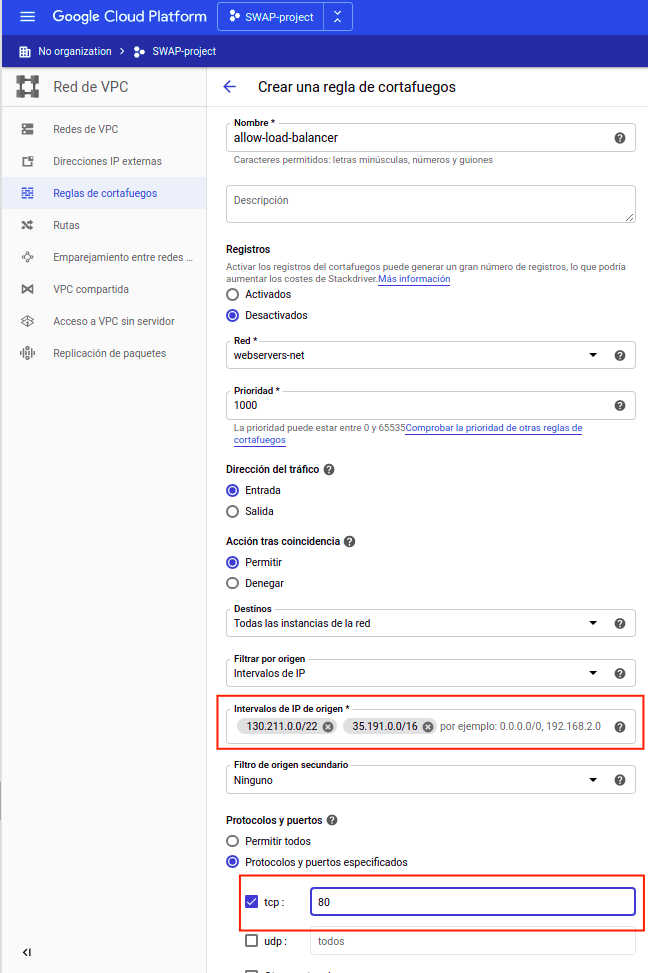
\includegraphics[width=0.5\textwidth]{project/firewall_balancer.png}
		\caption{Creación de la regla de firewall}
	\end{figure}
	\item Eliminamos la regla que creamos al principio (permitía conexiones desde cualquier lugar).
	\item Comprobamos que podemos acceder al balanceador pero no a las instancias mediante sus IPs externas:
	\begin{figure}[H]
		\centering
		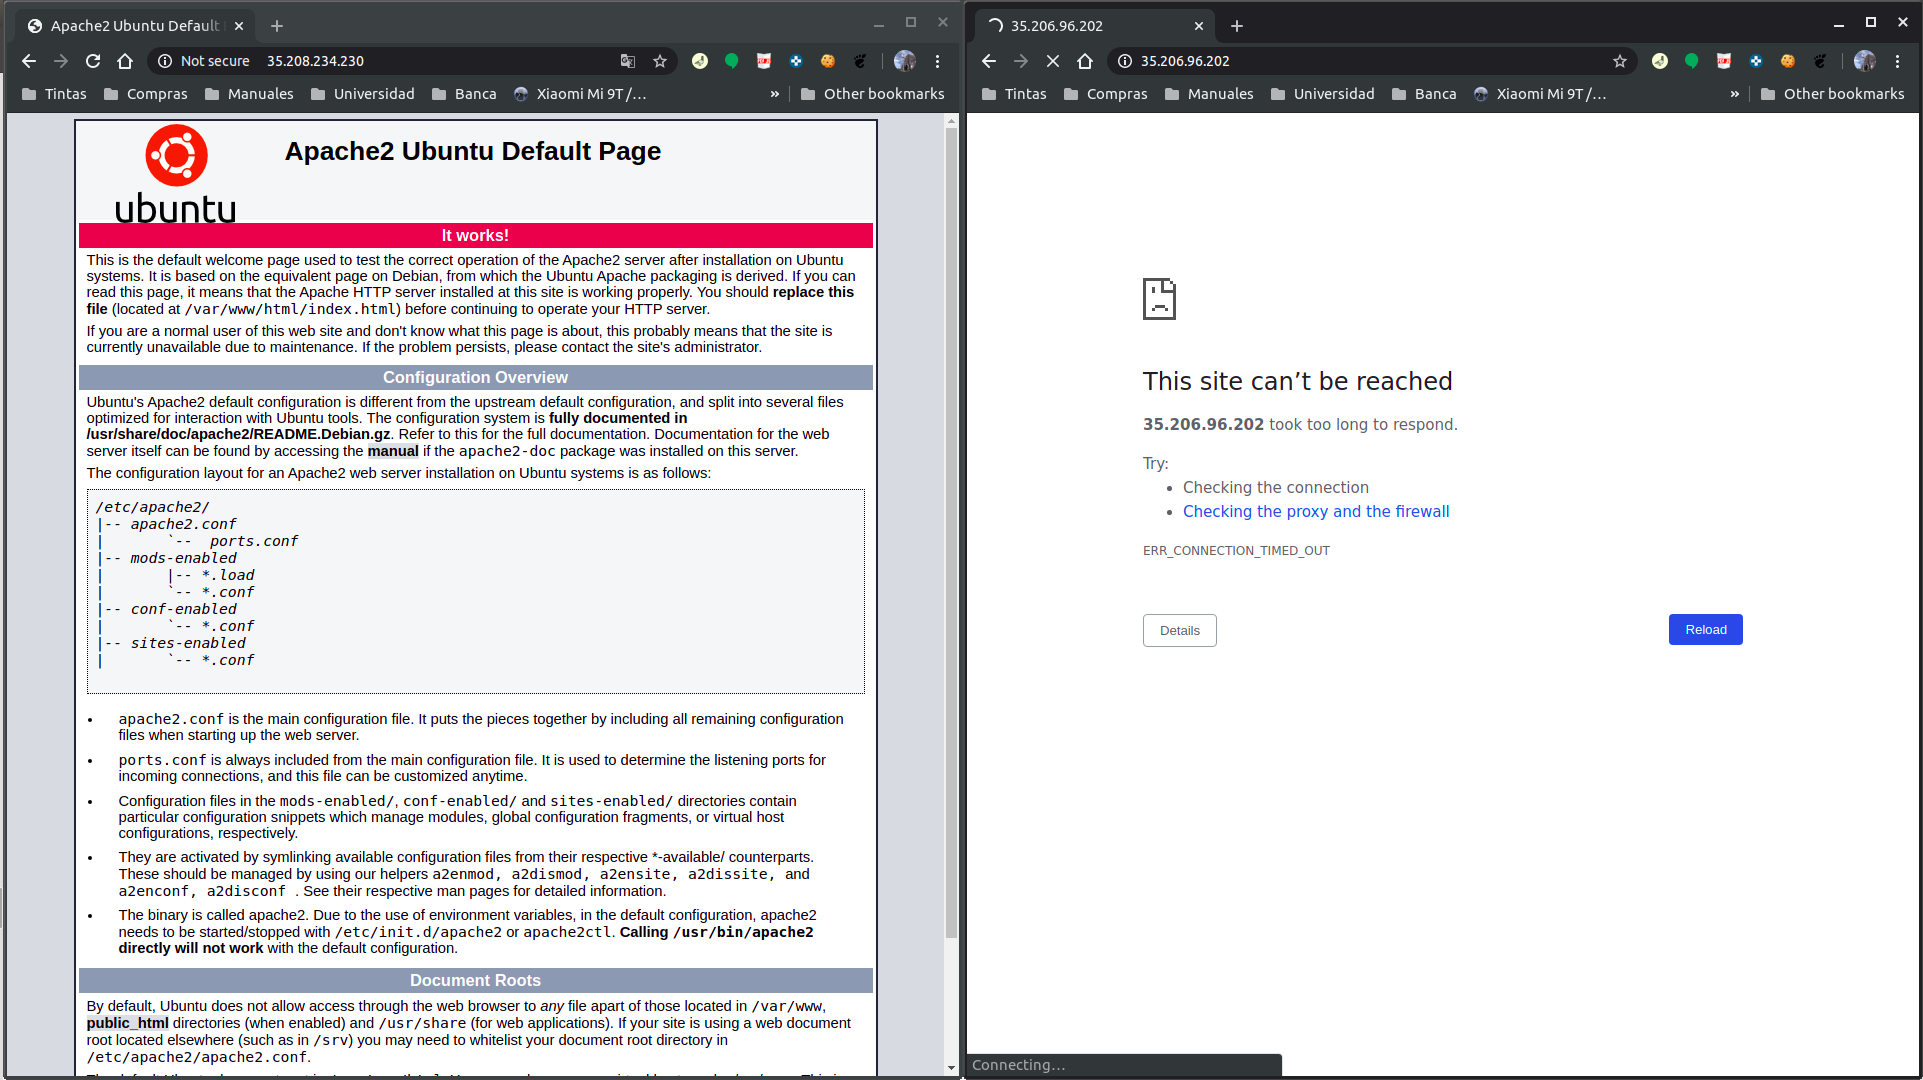
\includegraphics[width=\textwidth]{project/new_firewall_ok.png}
		\caption{Comprobación del funcionamiento del firewall}
	\end{figure}
\end{enumerate}

\section{Conclusiones}

Google Cloud Platform ofrece una forma muy sencilla para desplegar una arquitectura. Además, la gran cantidad de tutoriales que ofrece son muy útiles para hacerse al manejo de la plataforma.
\newpage
\bibliographystyle{apacite}
\nocite{*}
\bibliography{refs}






\end{document}
